% !TEX root = diplomarbeit.tex
\chapter{Firmware}
\renewcommand{\kapitelautor}{Autor: Christina Bornberg, Lucas Ullrich}

%%%%%%%%%%%%%%%%%%%%%%%%%%%%%%%%%%%%%%%%%%%%%%%%%%%%%%%%%%%%%%%%%%%%%%%%%%%%%%%
\section{Allgemeine technische Planung}

  \subsection{Konvention}
  In der Arbeit wird folgende Konvention festgelegt. Die z-Achse ist die Höhe, die y-Achse ist vorwärts und rückwärts und die x-Achse ist seitwärts.

  % BILD %

  \subsection{Tischplan}
  Das Konzept Tischplan beschreibt den Aufbau des Restaurants, also welche Komponenten benötigt werden und wo diese platziert sind.
  Um eine vorgegeben Route fliegen zu können muss dem Multicopter ein Routenplan bereitgestellt werden, in welchem die einzelnen Markierungspunkte enthalten sind, die der Multicopter auf seinem Weg zum Tisch überfliegt.

  Für den Tischplan wird die symbolische Positionierung genutzt. Er besteht aus folgenden Komponenten:

  \subsection*{Küche}
  Die Küche beschreibt den Bereich, in dem der Kellner interagiert. Hier befindet sich die Base, eine Plattform, die mit einem Farbcode ausgestattet ist. Auf ihr steht der Hexacopter und wartet auf die Beladung des auszuliefernden Cupcakes und den Befehl, loszufliegen.
  Das Admin Interface und der Server stehen ebenfalls in der Küche, über diese Komponenten bekommt der Hexacopter Befehle. Die Routen zu jedem Tisch sind im Admin Interface hinterlegt.

  \subsection*{Weg}
  Der Weg besteht, aus sich abwechselnden zweifarbigen Codes. Die Bereiche zwischen Tischen und Kreuzungen, werden als Wegabschnitt bezeichnet. Die ColorCodes müssen von jedem Restaurant eigenständig eingescannt und die Routen zum jeweiligen Tisch in das Admin Interface eingetragen werden.

  \subsection*{Tisch}
  Auf einem Tisch befindet sich, wie in der Küche, eine Plattform, die mit einem Farbcode versehen ist. Hier landet der Hexacopter, wartet 30 Sekunden lang und fliegt danach den Weg zurück zu seiner Base. In den 30 Sekunden soll der Cupcake entnommen werden. Weiters befindet sich ein iPad auf jedem Tisch. Durch dieses erhält jeder Tisch seine eigene ID und die dazugehörige Route. Bestellungen können somit einem Tisch zugewiesen werden.
  Die Tische können wie in jedem normalen Restaurant beliebig platziert werden, da der Hexacopter durch die Rotation der Farbobjekte auch Kurven fliegen kann. Dabei darf ein Teil des Tisches nicht besetzt sein, da die Drohne nicht über Menschen fliegen soll.

  % Bild vom Ablauf %%%%%%%%%%%%%%%%%%%%%%%%%%%%%%%%

  \subsection{Flussdiagramme}
  Für einen besseren Überblick über die einzelnen Programme und deren geforderten Funktionen wurden einzelne Flussdiagramme des gesamten Prozesses erstellt.
  Diese dienen nachfolgend als Orientierung beim Programmieren der einzelnen Funktionen.

  \begin{figure}[tbh]
    \begin{centering}
      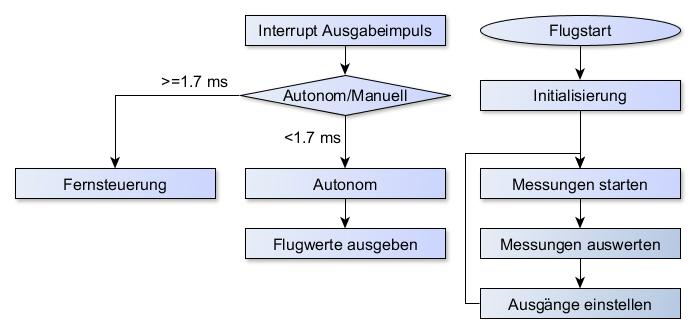
\includegraphics[width = \textwidth]{Bilder/Flussdiagramm}
    \par\end{centering}
    \caption{Flussdiagramm des Gesamtablaufs}
    \label{Flussdiragramm}
  \end{figure}

  Für die weiteren Programmteile wurden jeweils noch detailliertere Flussdiagramme erstellt.

%%%%%%%%%%%%%%%%%%%%%%%%%%%%%%%%%%%%%%%%%%%%%%%%%%%%%%%%%%%%%%%%%%%%%%%%%%%%%%%
\section{Navigation}

  \subsection{Technische Planung}

    \subsection*{Frames}
    Ein Frame entsteht bei jeder Messung der Pixy CMUcam5. Der Frame hat eine Breite von 319 und eine Höhe von 199 Pixel. Die Koordinate (0/0) befindet sich in der linken oberen Ecke.

    Bild 1 beschreibt den alten Frame, Bild 2 den aktuellen. Die Position des Objektes, beschreibt die zentralen x und y Positionen im Frame. Die Differenz entsteht aus den unterschiedlichen Positionen des Objektes im alten und neuem Frame. Das Objekt soll in den Bereich zwischen X\_MIN und X\_MAX, beziehungsweise Y\_MIN und Y\_MAX gelangen.

    % BILD VON LUCAS %

    \subsection*{Aileron}
    Anhand des aktuell getrackte Colorcodes wird die seitliche Position korrigiert. Solange sich der Hexacopter nicht im angegeben Bereich befindet, wird die Fluggeschwindigkeit in die jeweilige Richtung erhöht.

    \subsection*{Elevator}
    Durch den getrackten Colorcode, wird die Vorwärts- beziehungsweise Rückwärtsbewegung eingestellt. Die Position des Markers soll sich, wie bei der Bewegung nach Links und Rechts, in einem vorgegebenen Bereich befinden.
    Das Kamerasystem trackt den ersten Marker, bis er sich im richtigen Bereich befindet und der zweite Marker erkannt wird, dieser wird ebenfalls verfolgt, danach kommt der dritte. Diese Routine läuft, bis der letzte Colorcode erreicht ist. Im Idealfall muss die Rückwärtsbewegung während des Fluges gar nicht durchgeführt werden. Die Rückwärtsbewegung findet ihre Anwendung nur, wenn der Hexacopter beim letzten Farbcode angekommen ist und über sein Ziel hinausfliegt, oder, wenn kein nächster Farbcode gefunden wird. Welcher Marker der Zielmarker ist, kann durch die Größe des Arrays, in dem die Marker gespeichert werden, herausgefunden werden. Dieses wird mit den Daten, die im Admin-Interface hinterlegt sind und im Endeffekt vom Wlan-Modul empfangen werden, befüllt.

    \subsection*{Rudder}
    Mithilfe der Rudder Funktion muss der Winkel auf die aktuelle Positionsmarkierung ausgerichtet werden. Dabei ist eine Ungenauigkeit von 5 Grad in beide Richtungen erlaubt.

    Für die Rotation werden die Grundlagen negativer binärer Zahlen benötigt.

    \begin{itemize}
    \item \textbf{Binäre Zahlen ohne Vorzeichen}\\
    0000 0000 = 0, 1111 1111 = 255
    \item \textbf{Binäre Zahlen mit Vorzeichen} - Ein Bit wird für das Vorzeichen verwendet. \\
    0000 0001 = 1 -> 1000 0001 = -1, \\
    0111 1111 = 127 -> 1111 1111 = -127
    \item \textbf{Einerkomplement} - Beim Invertieren aller Bits entsteht eine negative Zahl \\
    0000 0000 = "+0" -> 1111 1111 = "-0" \\
    0111 1111 = 127 -> 1000 0000 = -127
    \item \textbf{Zweierkomplement}\\
    0000 0001 = 1 -> 1111 1111 = -1 \\
    0000 0010 = 2 -> 1111 1110 = -2 \\
    0111 1111 = 127 -> 1000 0001 = -127
    \item \textbf{Bilden des Zweierkomplements}\\
    \textbf{Beispiel:} 0111 1111 = 127 \\
    Die binäre Zahl wird invertiert (1000 0000) und mit 1 addiert. \\
    Das Ergebins lautet: 1000 0001 = -127 \\
    \textbf{Beispiel:} 1001 1000 = -104 \\
    Die binäre Zahl wird invertiert (0110 0111) und mit 1 addiert. \\
    Das Ergebnis lautet: 0110 1000 = 104 \\
    \end{itemize}

    % Bild von Rotation %

    \subsection*{Throttle}
    Über den Ultraschallsensor erfährt der Hexacopter, wie hoch er fliegt. Beim Erreichen der maximalen Flughöhe, wird seine Antriebskraft gesenkt. Dadurch korrigiert er seine Höhe bei jedem Aufruf der Funktion und eine Änderung des Gewichts, kann ausgeglichen werden. Der entnommene Cupcake und die damit verbundene Gewichtsveränderung stellt daher kein Problem dar.

  \subsection{Umsetzung}

    \subsubsection{Vergleichen der Frames}
    Für den Vergleich des aktuellen Frames mit dem letzten Frame, werden zwei \glslink{Struktur}{Strukturen} verwendet, die über folgende Mitglieder verfügt. \cite{Structs}
    \begin{itemize}
      \item \textbf{num} ist die ID des getrackten Colorcodes, er besteht aus einer zweistelligen Zahl.
      \item \textbf{pos\_x} ist die X-Position des Colorcodes. Der Wert bezieht sich auf das Zentrum des Objektes.
      \item \textbf{pos\_y} ist die Y-Position des Colorcodes. Der Wert bezieht sich auf das Zentrum des Objektes.
      \item \textbf{height} ist die, vom Ultraschall übergebene Höhe.
      \item \textbf{angle} ist die Rotation des Colorcodes. Da er zweifarbig ist, kann die PIXY CMUcam5 die Rotation des Objektes feststellen.
    \end{itemize}

    Zuerst wird die ID des Colorcodes verglichen, um herauszufinden, ob das Farbobjekt das selbe ist, wie im letzten Frame.
    Sollte dies der Fall sein, werden die Koordinaten x und y und die Rotation mit den Werten der älteren Struktur verglichen und in einer weiteren Strunktur gespeichert. Dieses wird bei den folgenden Funktionen verwendet, um anhand der Änderung zwischen zwei Frames zu überprüfen, ob der Hexacopter die richtige Geschwindigkeit hat.

    \subsubsection{Aileron, Elevator und Rudder anhand der Kameradaten}
    Durch die PIXY CMUcam5 kann die Position des Hexacopters, relativ zu einem Colorcode, festgestellt werden. Gegebenenfalls werden anschließend die Flugparameter verändert.

    \begin{figure} [tbh]
      \begin{centering}
        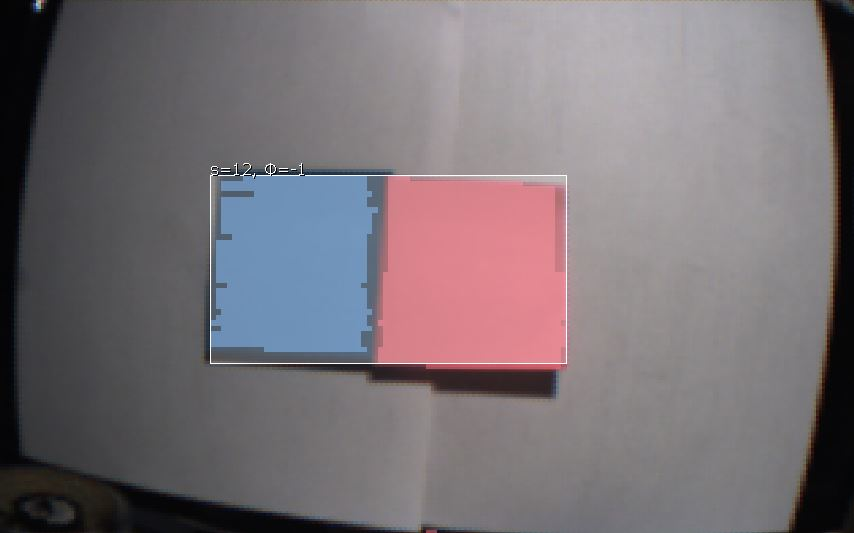
\includegraphics[width = \textwidth]{Bilder/Farbcode_erkannt}
      \par\end{centering}
      \caption{Ein erkannter Farbcode}
      \label{Farbcode_erkannt}
    \end{figure}
    Die Position wird anhand solcher Farbcodes erkannt, im Tischkonzept ist hinterlegt in welcher Reihenfolge der Hexacopter die Farbcodes suchen muss.
    Er fliegt anschließend so lange, bis er über dem aktuellen Farbcode ist, dieser also mittig im Bild ist und sucht darauf den nächsten.

    \subsubsection{Überprüfen von Aileron}
    Beim Vergleichen von Aileron wird die Veränderung an der x-Achse überprüft.

    Durch diese Funktion soll der Hexacopter mithilfe der Pixy-Daten, den Colorcode in der Mitte des Frames plazieren. An der x-Achse sind Werte zwischen 150 und 170 optimal. Der übergebene Wert ist dabei der Mittelpunkt des Colorcodes.
    Sollte die Pixycam keinen Wert in diesem Bereich erfassen, kann sie durch eine weitere Funktion namens ActAileron, welche die Änderungsrate an den Flightcontroller weitergibt, die Position an der x-Achse korrigieren.
    Um herauszufinden, ob der Mittelpunkt unter oder über dem optimalen Wert liegt, also der Hexacopter zu weit links oder rechts vom Objekt fliegt, gibt es für beide Fälle eine Abfrage.
    Um den Aileron Wert entgültig zu setzen, müssen nach der Überprüfung, ob der übergebene Wert an der x-Achse 170 überschreitet beziehungsweise 150 unterschreitet, folgende Zustände kontrolliert werden.
    Zunächst muss der Hexacopter über die Pixycam herausfinden, ob er sich bereits in die richtige Richtung bewegt. Dafür werden die beiden Frames miteinander verglichen. Wenn der Wert zu hoch ist, muss der x-Wert im alten Frame größer als im neuen sein. Sollte er zu niedrig sein, muss der Wert im neuen Frame höher sein.
    Anderenfalls fliegt der Hexacopter auf die falsche Seite. Die Firmware reagiert darauf mit der Änderung der Pulszeit am Aileron-Pin.
    Bei der Bewegung in die richtige Richtung wird der Wert so lange in diese gesteuert, bis sich die Geschwindigkeit, gemessen in den veränderten Pixel zwischen zwei Frames, zwischen zwei konstanten Werten befindet.

    \subsubsection{Überprüfen von Elevator}
    Elevator, die Bewegung an der y-Achse, also die Bewegung nach vorne und nach hinten, funktioniert nach dem selben Prinzip wie Aileron.

    Zuerst wird kontrolliert, ob sich der Farbcode im gewünschten Bereich befindet, in diesem Fall zwischen 90 und 110.
    Sollte der Mittelpunkt an der y-Achse nicht in diesem Bereich liegen, fliegt der Hexacopter nach vorne beziehungsweise zurück.
    Da die Route aus mehreren Farbcodes besteht, richtet sich der Hexacopter, sobald der Colorcode im Bereich zwischen 90 und 100 liegt, nach dem Objekt, das sich am nächsten zum Nullpunkt der y-Achse befindet. Somit probiert er die Position zentriert über dem Farbobjekt zu optimieren, bis er das nächste Farbobjekt erkennt und trackt. Das alte Objekt ist nun unwichtig, der Hexacopter bezieht sich auf das vordere Farbobjekt.

    Wie bei der Überprüfung von Aileron, gibt es auch hier zwei konstante Werte, zwischen denen sich die Geschwindigkeit befinden soll, solange die Position optimiert wird.

    \subsubsection{Überprüfen von Rudder}
    Rudder beschreibt die Rotation um seine eigene Hochachse. Dafür wird zunächst unterschieden, ob sich der Hexacopter am Hin- oder Rückflug befindet, da die Rotation der Colorcodes beim Rückflug um 180 Grad gedreht werden muss.

    Die optimale Rotation befindet sich beim Hinflug zwischen -5 und 5 Grad.
    Bei einem zu niedrigen oder zu hohen Wert wird kontrolliert, ob sich der Hexacopter bereits in die richtige Richtung dreht.
    Sollte dies nicht der Fall sein, wird die Änderungsrate an die dazugehörige Funktion geschickt, die dem Flightcontroller die Information zur Beschleunigung gibt.
    Ansonsten wird die Veränderung der Pixel zweier Frames verglichen, wenn sie sich im gewünschten Bereich befindet, wird der Wert nicht geändert, bei einem zu hohen Wert, wird die Rotationsgeschwindigkeit gesenkt, ansonsten erhöht.

    Beim Rückflug soll die Rotation des Colorcodes größer als 175 oder kleiner als -175 sein.

    \subsubsection{Throttle anhand des Ultraschallsensors}
    Der Hexacopter steht auf einer Landeplattform in seiner Base. Unter ihm ist ein Farbcode, den er so lange fokusiert, bis er den nächsten Farbcode trackt. Den zweiten Farbcode kann er erst scannen, wenn er hoch genug fliegt um an der Tischkante vorbei, den nächsten Farbcode zu scannen.

    Beim Starten fliegt er vertikal nach oben, bis er den zweiten Farbcode erkennt. Um beim Start nicht abzudriften, beschleunigt er, solange er sich unter einer Höhe von $\SI{50}{\centi\metre}$ befindet, mit einer hohen Änderungsrate. Ab dieser Höhe beschleunigt er mit einer geringeren Erhöhung der Änderungsrate, bis er die $\SI{80}{\centi\metre}$-Grenze erreicht hat.
    zwischen $\SI{80}{\centi\metre}$ und $\SI{120}{\centi\metre}$ bleibt die Beschleunigung gleich, das führt jedoch dazu, dass der Hexacopter den oberen Rand von $\SI{120}{\centi\metre}$ erreichen wird, da er bis jetzt nicht gebremst wird. Sobald er über $\SI{120}{\centi\metre}$ kommt, wird die Beschleunigung reduziert. Der Hexacopter pendelt sich zwischen $\SI{80}{\centi\metre}$ und $\SI{120}{\centi\metre}$ ein.

    Nun wird berechnet, ob er sich noch über dem Tisch oder schon über dem Boden befindet. Dies stellt er fest, wenn zwei hintereinanderliegende Messungen einen Höhenunterschied von $\SI{50}{\centi\metre}$ aufweisen. Die zweite Messung ist erforderlich, um mögliche Fehlmessungen auszuschließen.

    Wenn er nun über dem Boden fliegt, beträgt seine minimale Höhe $\SI{180}{\centi\metre}$ und seine maximale Höhe $\SI{220}{\centi\metre}$.
    Der Hexacopter beschleunigt nach dem selben Prinzip, wie über einem Tisch. Unter $\SI{100}{\centi\metre}$ ändert er seine Beschleunigung mit einem hohen Wert. Bis $\SI{180}{\centi\metre}$ beschleunigt er mit einer niedrigeren Änderungsrate. Sollte der Hexacopter über $\SI{220}{\centi\metre}$ fliegen, wird die Beschleunigung durch eine negative Änderungsrate gesenkt.

    Der Hexacopter fliegt mit diesen Werten, bis er den vorletzten Farbcode erreicht hat. Da die Farbcodes in einem Array abgespeichert werden, ist die Anzahl der darin gespeicherten Farbcodes bekannt.

    Beim letzten Farbcode angekommen, also dem am Tisch liegenden Farbcode, wird ebenfalls wieder durch die Kontrolle von zwei Werten, die sich um $\SI{50}{\centi\metre}$ von der vorigen Messung unterscheiden müssen, analysiert, wann sich der Hexacopter über dem Tisch befindet. Sobald dies der Fall ist, landet er, indem er die Beschleunigung mit einer negativen Änderungsrate verlangsamt. Dabei muss er sich, zwischen einer vom System vorgegebenen Mindest- und Maximalgeschwindigkeit, befinden.

    Nach der Landung wird die Routeninformation umgekehrt, der erste Colorcode wird zum letzten, der zweite zum vorletzten und so weiter. Außerdem muss die Rotation der Farbcodes beim Rückflug um 180 Grad gedreht sein, dafür wird die Richtung als Rückflug abgespeichert. Sollte sich der Hexacopter wieder in der Base befinden, wird die Variable wieder als Hinflug gespeichert.

    Damit genügend Zeit für das herunternehmen des Cupcakes ist, verweilt der Hexacopter eine halbe Minute am Tisch, bevor er seinen Rückflug antritt.

    \subsubsection{Speichern der alten Daten}
    Die alten Daten werden gespeichert, um die Differenzen von zwei Frames zu errechnen. Der Frame mit Index 0, ist der aktuelle Frame, der Frame mit dem Index 1, der alte. Bei jedem Durchlauf, werden die Werte aktualisiert.

    \subsubsection{Ausgabe der Steuersignal}
    Autor: Lucas Ullrich\\
    Nachdem die Steuersignale berechnet und korrigiert wurden, müssen diese an den Hexacopter ausgegeben werden. Dies muss periodisch alle $\SI{20}{\milli\second}$ geschehen.
    Der Flightcontroller erkennt jeweils die einzelnen Impulse und steuert die Rotoren entsprechend an.

    Diese Impulse werden interruptgesteuert ausgegeben, der Interrupt wird von dem Gear-Pin erzeugt, welcher gleichzeitig für den Flugmodus verantwortlich ist.

    \lstset{language = c}
    \begin{lstlisting}
interrupt void Isr() {
  if(CCP1IF == 1) {
    CCP1IF = 0;
    T1CONbits.TMR1ON = 0;
    SignalOut();
    NOP();
  }
  if(TMR3GIF == 1) {
    TMR3GIF = 0;
    ModeCheck();
    SignalOut();    /* initial call after remaining break to 20 ms
                     * starts with Aileron (needs to be set in last
                     * case statement, case 0) following delays will
                     * be processed by the previous routine */
    pulsecounter++;
  }
}

void SignalOut(void) {
  switch(pin_out) {
    case 'A': {
      A = 1;
      Delay(a_actors[0].aile);
      pin_out = 'E';
      break;
    }case 'E': {
      A = 0;
      E = 1;
      Delay(a_actors[0].elev);
      pin_out = 'T';
      break;
    }
    \end{lstlisting}
    Die weiteren Signale (Throttle und Rudder) werden auf die gleiche Weise ausgegeben.
    Die Delay-Funktion stellt die Compare-Einheit so ein, dass nach der gewünschten Pulsdauer des Ausgangs ein Interrupt hervorgerufen wird.

%%%%%%%%%%%%%%%%%%%%%%%%%%%%%%%%%%%%%%%%%%%%%%%%%%%%%%%%%%%%%%%%%%%%%%%%%%%%%%%
\section{Objekterkennung Lucas}
Die Objekterkennung ist für den Hexacopter notwendig um eine zuverlässige Positionierung zu ermöglichen. Dazu werden bestimmte Objekte im Raum erkannt und als Orientierung
genutzt oder es muss ihnen ausgewichen werden \bzw eine Kollision vermieden werden.

  \subsection{Technische Planung}
  In der Planung war es wichtig einerseits die notwendige Rechenleistung gering zu halten, andererseits auch alle notwendigen Objekte erkennen zu können.

  \subsection{Umsetzung}

  \subsection{Herausforderungen und Lösungen}

%%%%%%%%%%%%%%%%%%%%%%%%%%%%%%%%%%%%%%%%%%%%%%%%%%%%%%%%%%%%%%%%%%%%%%%%%%%%%%%
\section{Sicherheit}

  \subsection{Technische Planung}

Sicherheitskonzepte

Beim Konzept Sicherheitsmaßnahmen geht es grundsätzlich um die Sicherheit von Mensch, Umgebung und dem Multicopter selbst. Hier werden mögliche Fehler mit Anlehnung an FMEA ("Fehlermöglichkeits- und -einflussanalyse" / "Auswirkungsanalyse") analysiert. Dieses Konzept ist ein rein schriftliches Konzept.

  \subsection{Umsetzung}

    Legende:
    \begin{itemize}
    \item A: Auftreten
    \item B: Bedeutung
    \item E: Entdeckung
    \item RPZ: Risiko-Prioritätszahl = A * B * E
    \end{itemize}

    Die Werte beziehen sich auf den Fehler, die obere Analyse beschreibt das Auftreten, die Bedeutung und die Entdeckung vor den Maßnahmen, die unteren nach den Maßnahmen.

%\begin{table}[H]
%\centering
\begin{longtable}{|p{0.4cm}|p{3.0cm}|p{3.1cm}|p{3.1cm}|p{0.4cm}|p{0.4cm}|p{0.4cm}|p{0.8cm}|}

\hline \#   & Bezeichnung                                                                                               & Fehler                                                                                                                & Beschreibung                                                                                                                    & A   & B   & E   & RPZ \\
 1          & Mensch in unmittelbarer Nähe                                                                              & Mensch wird verletzt, da Hexacopter nicht ausweicht                                                                   & Eine Person steht auf dem Weg und wird vom Hexacopter als Hindernis erkannt                                                     & 5   & 10  & 10  & 500 \\
\hline -    & Vermeidung                                                                                                & Maßnahme nach Eintritt                                                                                                & Mögliche Softwarelösung                                                                                                         & A   & B   & E   & RPZ \\
 -          & Wege absperren, Menschen darauf hinweisen, sich nicht in unmittelbarer Nähe des Hexacopters aufzuhalten.  & Hexacopter landet auf der Stelle um die Sicherheit der Person zu gewährleisten.                                       & Durch 2 Ultraschallsensoren, die vorne am Hexacopter angebracht sind, werden Menschen erkannt, er landet daraufhin.             & 2   & 10  & 5   & 100 \\\hline

\hline \#   & Bezeichnung                                                                                               & Fehler                                                                                                                & Beschreibung                                                                                                                    & A   & B   & E   & RPZ \\
 2          & Ein unbewegliches Hindernis befindet sich in unmittelbarer Nähe.                                          & Hexacopter fliegt gegen ein unbewegliches Hindernis und stürzt ab.                                                    & Eine Wand oder ein ähnliches unbewegliches Hindernis befindet sich in unmittelbarer Nähe.                                       & 5   & 7   & 9   & 315 \\
\hline -    & Vermeidung                                                                                                & Maßnahme nach Eintritt                                                                                                & Mögliche Softwarelösung                                                                                                         & A   & B   & E   & RPZ \\
 -          & Farbcodes werden nicht in der Nähe von unbeweglichen Hindernissen platziert.                              & Der Hexacopter landet, da er nicht zwischen Mensch, beweglichen und unbeweglichen Hindernissen unterscheiden kann.    & Der Hexacopter darf nur über Farbcodes fliegen, dadurch wird vermieden, dass der Hexacopter in die Nähe dieser Objekte kommt.   & 1   & 7   & 5   & 35  \\\hline

\hline \#   & Bezeichnung                                                                                               & Fehler                                                                                                                & Beschreibung                                                                                                                    & A   & B   & E   & RPZ \\
 3          & Bewegliches Hindernis wird erkannt                                                                        & Hexacopter fliegt gegen ein Hindernis und stürzt ab                                                                   & Eine Hindernis wird erkannt.                                                                                                    & 3   & 6   & 10  & 180 \\
\hline -    & Vermeidung                                                                                                & Maßnahme nach Eintritt                                                                                                & Mögliche Softwarelösung                                                                                                         & A   & B   & E   & RPZ \\
 -          & Bewegliche Hindernisse werden wenn möglich aus dem Weg geräumt.                                           & Hexacopter probiert dem Hindernis auszuweichen und seinen Weg weiter zu meistern.                                     & Durch 2 Ultraschallsensoren, die vorne am Hexacopter angebracht sind, werden Hindernisse erkannt, er landet daraufhin           & 2   & 6   & 5   & 60  \\\hline

\hline \#   & Bezeichnung                                                                                               & Fehler                                                                                                                & Beschreibung                                                                                                                    & A   & B   & E   & RPZ \\
 4          & Hände in der Nähe von den Propellern                                                                      & Person hat seine Hände beim fliegenden Hexacopter und verletzt sich                                                   & Eine Person greift in die Propeller.                                                                                            & 7   & 10  & 10  & 700 \\
\hline -    & Vermeidung                                                                                                & Maßnahme nach Eintritt                                                                                                & Mögliche Softwarelösung                                                                                                         & A   & B   & E   & RPZ \\
 -          & Hexacopter wartet lang genug, dass man den Cupcake runternehmen kann. Propellerschutz ist angebracht.     & Hexacopter gibt über Display / LED / Ton aus, dass er wegfliegt.                                                      & Display / LED / Ton werden programmiert um Menschen beim Start zu warnen.                                                       & 1   & 10  & 5   & 50  \\\hline
 \caption{Fehlt noch}
\end{longtable}
%\end{table}


%%%%%%%%%%%%%%%%%%%%%%%%%%%%%%%%%%%%%%%%%%%%%%%%%%%%%%%%%%%%%%%%%%%%%%%%%%%%%%%
\section{Systemausfall}

Das Konzept Systemausfall beschreibt die Maßnahmen, wenn der Hexacopter seine Anforderungen nicht erfüllen kann. Dieses Konzept ist rein schriftlich entwickelt.

  \subsection{Technische Planung}

  Mögliche Ursachen: \cite{tech_def}
  \begin{itemize}
  \item Materialermüdung
  \item Programmfehler (eingespeiste Daten, Programmablauffehler)
  \item menschlicher Fehler
  \item falsche Montage
  \item fehlender elektrischer Kontakt
  \item unzureichende oder fehlende Energieversorgung
  \item Fehler in der Datenverarbeitung; beispielsweise Datenübertragung, Informationsverlust, Rechenfehler
  \end{itemize}


  \subsection{Umsetzung}
  Mit einem Stern gekennzeichnete Fehler, sind in der Firmware berücksichtigt.

\begin{table}[H]
\centering
\begin{tabular}{|p{7cm}|p{7cm}|}
\hline Fehler & Lösung\\\hline
\hline Akku schwach & Fail Safe, eventuell sofort landen\\
\hline Akku explodiert: Lithium Ionen Akkus können explodieren & Vor dem Flug kontrollieren, Feuerlöscher bereitstellen\\
\hline Copter findet keine Farbobjekte mehr & Position Hold, nach einer Zeit: Landen\\
\hline Copter findet falsche Farbobjekte & Position Hold, nach einer Zeit: Landen \\
\hline Ausfall von Aktoren (Propeller, bzw. Motoren blockiert/ …) &  Wenn es möglich ist: Landen\\
\hline Copter fliegt in die falsche Richtung * & Da Colorcodes aus 2 Farben bestehen, kann die Rotation des Objektes bestimmt und korrigiert werden. \\
\hline Hexacopter ist zu hoch / verliert an Höhe * & Durch die Daten des Ultraschallsensors, kann die Höhe korrigiert werden.\\
\hline Ausfall von Sensoren (Pixy / Ultraschall / …) & Fehlermeldung, Manueller Flug\\
\hline Hackerangriff & Durch den WLAN Standard (wpa2) ist die Übertragung sicher genug\\
\hline Funkstörung bei manuellem Flug & Pilot muss verstehen, in welchem Frequenzband die Fernsteuerung arbeitet, Störquellen vermeiden und abschalten (sonstiges WLAN, Bluetooth, andere Fernsteuerungen im Umfeld) -> saubere Vorbereitung - Analyse von möglichen Störquellen\\
\end{tabular}
\caption{Fehlt noch}
\end{table}

\subsection*{Beispiele für Lösungen}
\begin{itemize}
\item \textbf{Landen:} sofort auf der Stelle landen
\item \textbf{Position hold:} in der Luft stehen bleiben – Option auf manuelle Steuerung umstellen
\item \textbf{Fail Safe:} zurück zur Base fliegen und Flug abbrechen
\item \textbf{Manuell fliegen:} auf manuelle Fernsteuerung umschalten
\item \textbf{Fehlermeldung:} Fehlermeldung wird über Display oder blinkende LEDs ausgegeben. Fehler wird an Server gesendet
\end{itemize}

\subsection*{Was passiert nach einem Systemausfall?}
Wenn der Hexacopter seinen Fehler selbst korrigieren kann, fliegt er seine Route weiter.
Anderenfalls geht der Hexacopter, sobald er gelandet ist oder manuell gesteuert wurde, davon aus, beim nächsten Start in seiner Base zu stehen. Der Cupcake wird wieder in der Bestellliste angezeigt und muss erneut ausgeliefert werden. Je nach Fehler, wird ein Code über den Display ausgegeben, der bei der Fehlersuche helfen soll.
